\documentclass[12pt]{article}

\usepackage[a4paper,margin=2.5cm]{geometry}
\usepackage{amsmath, amssymb, amsthm}
\usepackage{bm}
\usepackage{hyperref}
\usepackage{graphicx}
\usepackage{caption}
\usepackage{listings}
\usepackage{xcolor}
\usepackage{float}
\usepackage{placeins}
\graphicspath{{figures/}}

\lstdefinestyle{code}{
  basicstyle=\ttfamily\small,
  numbers=left,
  numberstyle=\tiny,
  numbersep=8pt,
  keywordstyle=\color{blue},
  commentstyle=\color{teal!70!black},
  stringstyle=\color{orange!70!black},
  showstringspaces=false,
  breaklines=true,
  frame=single,
  framerule=0.3pt,
  rulecolor=\color{black!15}
}
\lstset{style=code}

\title{Hierarchical Clustering Tutorial}
\author{}
\date{\today}

\begin{document}
\maketitle

\section{Introduction}
Hierarchical clustering builds a multi-resolution view of data by successively merging or splitting clusters without pre-specifying their number. Agglomerative (bottom-up) methods start with singletons and iteratively merge the closest clusters using linkage criteria such as single, complete, average, or Ward's linkage. The resulting dendrogram captures nested structure, allowing practitioners to choose cluster counts post hoc by cutting the tree at different heights.

\section{Theory and Formulas}
\subsection{Linkage Functions}
For two clusters \(A\) and \(B\) with elements \(\mathbf{x}_i\) and \(\mathbf{x}_j\), popular linkage definitions include
\begin{align}
\text{single}(A,B) &= \min_{\mathbf{x}_i \in A,\, \mathbf{x}_j \in B} \lVert \mathbf{x}_i - \mathbf{x}_j \rVert_2,\\
\text{complete}(A,B) &= \max_{\mathbf{x}_i \in A,\, \mathbf{x}_j \in B} \lVert \mathbf{x}_i - \mathbf{x}_j \rVert_2,\\
\text{average}(A,B) &= \frac{1}{|A|\,|B|} \sum_{\mathbf{x}_i \in A} \sum_{\mathbf{x}_j \in B} \lVert \mathbf{x}_i - \mathbf{x}_j \rVert_2,\\
\text{Ward}(A,B) &= \frac{|A|\,|B|}{|A|+|B|} \lVert \bm{\mu}_A - \bm{\mu}_B \rVert_2^2,
\end{align}
where \(\bm{\mu}_A\) and \(\bm{\mu}_B\) are centroids. Ward's linkage minimizes the increase in within-cluster variance at each merge.

\subsection{Agglomerative Algorithm}
A generic agglomerative procedure is:
\begin{enumerate}
  \item Initialize each point as a singleton cluster and compute all pairwise distances.
  \item Repeatedly merge the pair of clusters with minimal linkage distance.
  \item Update the distance matrix using the chosen linkage rule.
  \item Continue until all samples form one cluster or a stopping criterion is met.
\end{enumerate}
The merge history forms a hierarchy encoded in the dendrogram's branching structure. Cutting the dendrogram at height \(h\) yields clusters with maximum within-cluster dissimilarity bounded by \(h\).

\subsection{Cophenetic Distance}
The cophenetic distance between points \(i\) and \(j\) is the dendrogram height at which they merge. Comparing the cophenetic correlation with the original distance matrix helps assess how faithfully the hierarchy preserves pairwise relationships.

\section{Applications and Tips}
\begin{itemize}
  \item \textbf{Taxonomy and phylogeny}: dendrograms naturally express hierarchical relationships among species or document categories.
  \item \textbf{Market basket analysis}: hierarchical clustering on products uncovers nested groupings useful for recommendation and shelf planning.
  \item \textbf{Feature engineering}: dendrogram cuts at different heights provide multi-scale cluster labels or grouping constraints for other algorithms.
  \item \textbf{Best practices}: standardize features, choose linkage consistent with data geometry, and watch for chaining (single linkage) or sensitivity to outliers (complete linkage).
\end{itemize}

\section{Python Practice}
The script \texttt{gen\_clustering\_hierarchical\_clustering\_figures.py} generates synthetic blobs, computes an agglomerative clustering, and saves both a dendrogram and a 2D scatter plot colored by cluster labels obtained from cutting the tree.
\begin{lstlisting}[language=Python,caption={Excerpt from gen_clustering_hierarchical_clustering_figures.py}]
from scipy.cluster.hierarchy import dendrogram, linkage, fcluster

linkage_matrix = linkage(points, method="ward")
labels = fcluster(linkage_matrix, t=3, criterion="maxclust")

# Plot dendrogram and colored scatter of assigned clusters
\end{lstlisting}

\section{Result}
\begin{figure}[H]
  \centering
  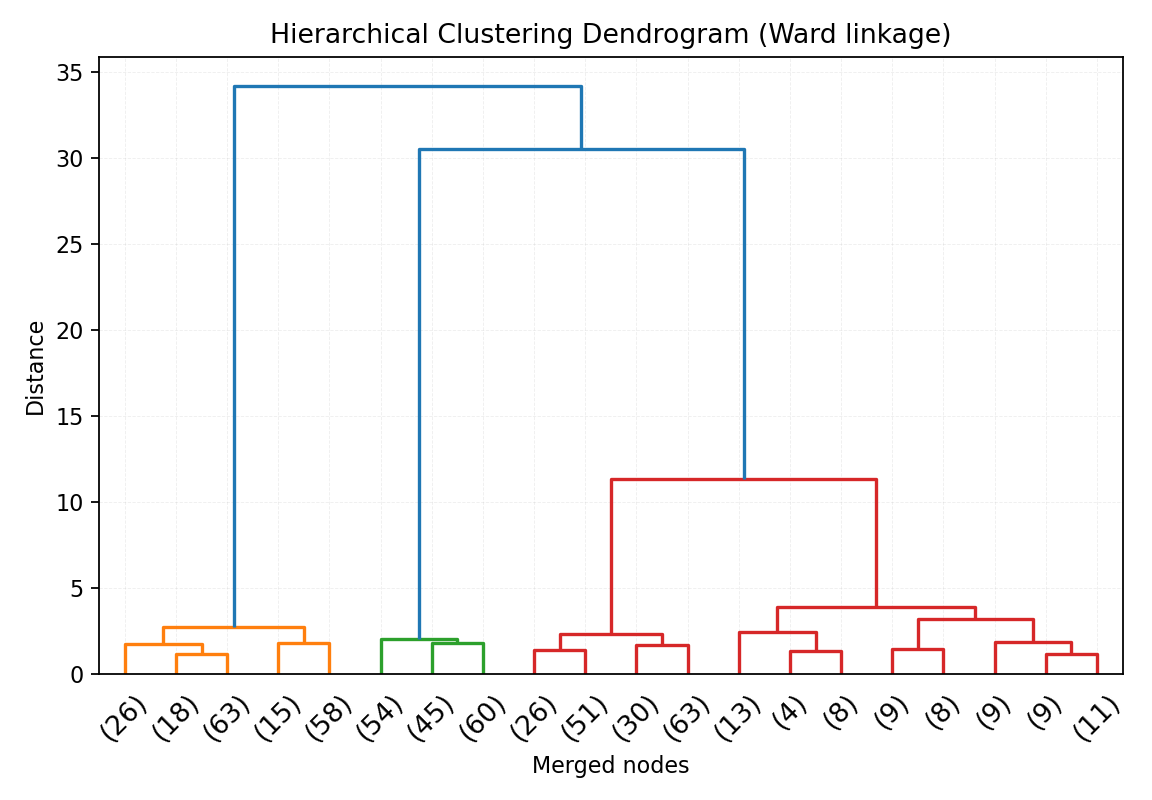
\includegraphics[width=0.85\linewidth]{hierarchical_dendrogram.png}
  \caption{Dendrogram produced by Ward linkage on synthetic blobs}
  \label{fig:hierarchical_dendrogram}
\end{figure}

\begin{figure}[H]
  \centering
  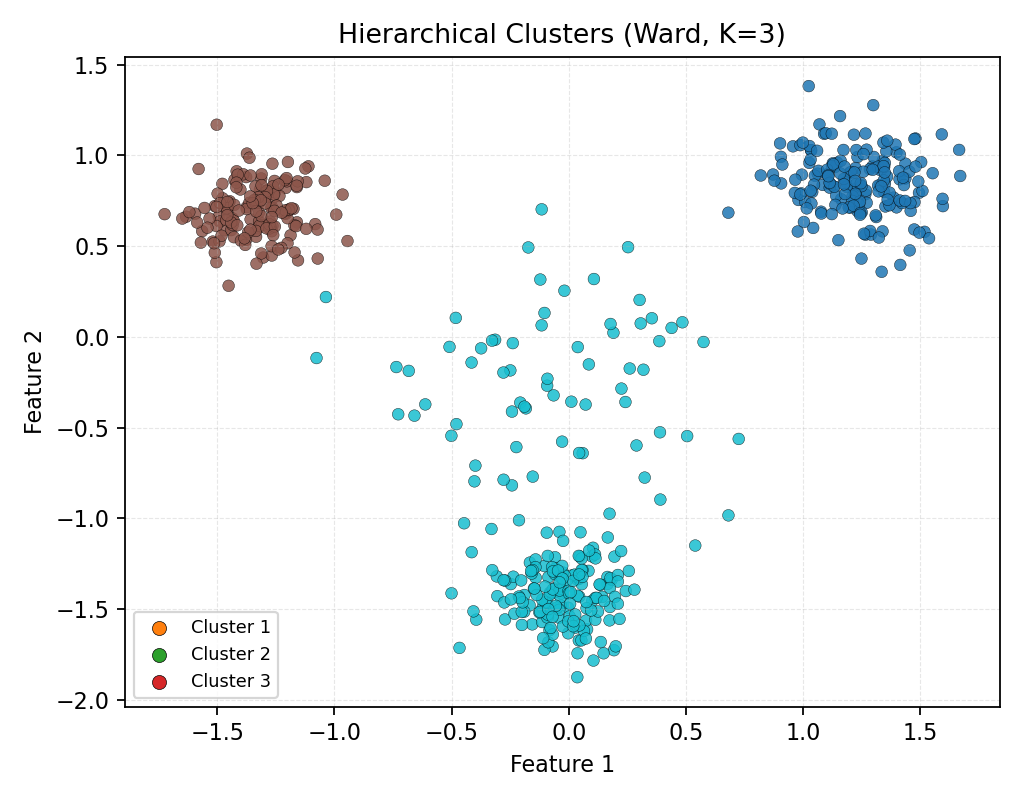
\includegraphics[width=0.82\linewidth]{hierarchical_clusters.png}
  \caption{Cluster assignments obtained by cutting the dendrogram at three clusters}
  \label{fig:hierarchical_clusters}
\end{figure}

\FloatBarrier
\section{Summary}
Hierarchical clustering reveals nested structure without committing to a fixed number of clusters upfront. Linkage choices control behavior: Ward favors compact clusters, average balances chaining and tightness, while single and complete emphasize connectivity extremes. The example demonstrates how dendrogram visualization and cluster cuts complement one another in exploratory analysis.

\end{document}
